\chapter{Sociale robotter}
\label{SocialRobot}
%
I det følgende kapitel vil der først blive specificeret hvad der karakteriserer en social robot og herunder belyses det hvilke eksisterende sociale robotter, der allerede er på markedet. Dernæst vil projektsamarbejdet blive yderlige specificeret. Efterfølgende fokuseres der på teknologier i lufthavne, hvorefter interaktion og udfordringer ved sociale robotter belyses. Afslutningsvist ledes der over i en problemformulering, som danner grundlag for det fremadrettede projektarbejde.
%
\section{Karakterisering af social robot}
\label{KarakteriseringAfSocialRobot}
%
Sociale robotter adskiller sig fra industrielle robotter, da det overordenede formål er, at de skal tage sig af mennesker, \parencite[s. 13]{PDF:RobotShiftFromIPtoSR}. Sociale robotter skal særligt tage sig af de svage i samfundet; ældre, handicappede, syge og børn, \parencite[s. 14]{PDF:RobotShiftFromIPtoSR}. Formålet med industrielle robotter er, at de kan udfører farligt og gentagende arbejde, hvorfor de potentielt kan rede menneskeliv, \parencite[ss. 12-13]{PDF:RobotShiftFromIPtoSR}. På \autoref{fig:CategorizationOfRobots} illustreres en kategorisering af robotter, hvor det blandt andet fremgår at industrielle robotter og sociale robotter ikke tilhører den samme robottype.    
%
\begin{figure}[H]
\centering
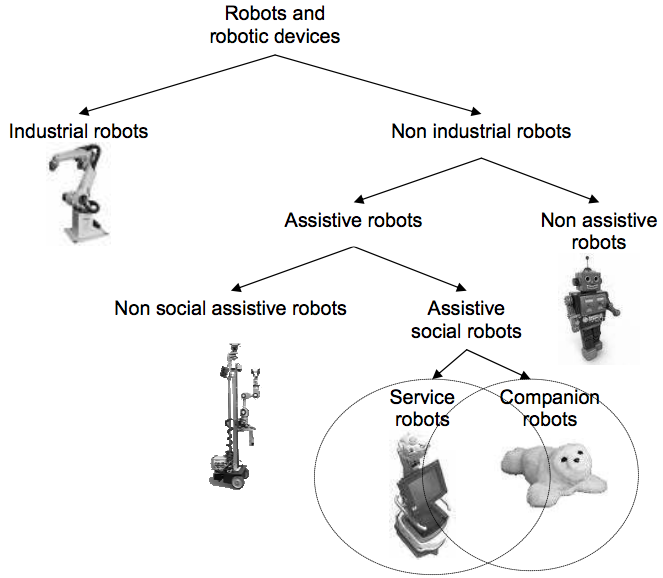
\includegraphics[width = 0.75\textwidth]{Figure/CategorizationOfRobots} 
\caption{Kategorisering af robotter fremsat af \textcite[s. 13]{PDF:AssesingAcceptance}.}
\label{fig:CategorizationOfRobots}
\end{figure}
\noindent 
%
Da projektet fokuserer på sociale robotter, \textit{Assistive social robots}, som skal indgå i en kontekst blandt mennesker, afgrænses der fra industrielle robotter, \textit{Non assistive robots} samt \textit{Non social assistive robots}. Sidste nævnte robottype er en form for fysisk teknologisk hjælpemiddel, der kan anvendes til rehabilitering, det kan eksempelvis være proteser eller intelligente kørestole, \parencite[s. 12]{PDF:AssesingAcceptance}.    

Ifølge \textcite[s. 1]{PDF:SharingALifeHarvey} kan sociale robotter karakteriseres ved, at de har forståelse og evne til at kommunikere på en menneskeagtig måde, hvilket gør det muligt for deres brugere at forstå dem. I tillæg argumenterer \textcite[s. 168]{PDF:TowardSociableRobots} for, at når mennesker enten observerer eller interagerer med en autonom robot tildeles den en social model. For at autonom robot kan kategoriseres som en social robot skal den, ifølge \textcite[s. 168]{PDF:TowardSociableRobots}, percipere omgivelserne, tage selvstændige beslutninger og udføre koordinerede handlinger for at løse deres opgave. Da sociale robotter designes til at interagere med mennesker, via simpel kommunikation, vil det øge brugerens accept af robotten, \parencite[s. 1476]{PDF:ExploringInfluencingVariable}. Ydermere forudser \textcite[s. 1476]{PDF:ExploringInfluencingVariable}, at sociale robotter i højere grad vil penetrerer vores hverdagsliv, hvorfor det er nødvendigt at undersøge, hvordan mennesket perciperer sociale robotter og hvorfor de enten accepterer eller afviser dem, \parencite[s. 1]{PDF:SharingALifeHarvey}.  



